\documentclass[11pt]{article}
\usepackage[utf8]{inputenc}
\usepackage[a4paper, margin=1in]{geometry}
\usepackage[parfill]{parskip} 
\usepackage{fancyhdr}
\usepackage{amsmath}
\usepackage{amsthm}
\usepackage{amssymb}
\usepackage{graphicx}
\usepackage{ragged2e}
\usepackage{mathtools}
\usepackage[utf8]{inputenc}
\usepackage{float}
\usepackage{xcolor}
\usepackage{subcaption}
\usepackage{booktabs}
\usepackage{array,multirow}
\usepackage{hyperref}
\usepackage{minted}
\usemintedstyle{monokai}


\title{\huge Programming Assignment 3: CS 747}


\author{\Large Richeek Das : 190260036}

\date{\textbf{2nd November 2021}}

\begin{document}
    
    \maketitle
    
    \pagenumbering{arabic} 
    \pagestyle{fancy}
    \fancyhf{}
    \lhead{190260036}
    \rhead{Assignment 3}
    \cfoot{Page \thepage}
    \renewcommand{\footrulewidth}{1pt}
    
    \renewcommand{\labelenumi}{(\alph{enumi})}
    \renewcommand{\labelenumii}{(\arabic{enumii})}
    
    \tableofcontents{}
    
    \vfill
    
    \begin{center}
        
\includegraphics[scale=0.30]{iitb.pdf}
  
        \vspace{0.5cm}
        {\normalsize
            Department of Computer Science and Engineering \\
            Indian Institute of Technology Bombay  \par}
        
        {\normalsize 2021-2022 \par}
        \vspace{0.5cm}
    \end{center}
    
    \pagebreak
    
    \section{\texttt{Task 1: "Tabular" Sarsa}}
    
    \begin{figure}[htbp!]
        \centering
        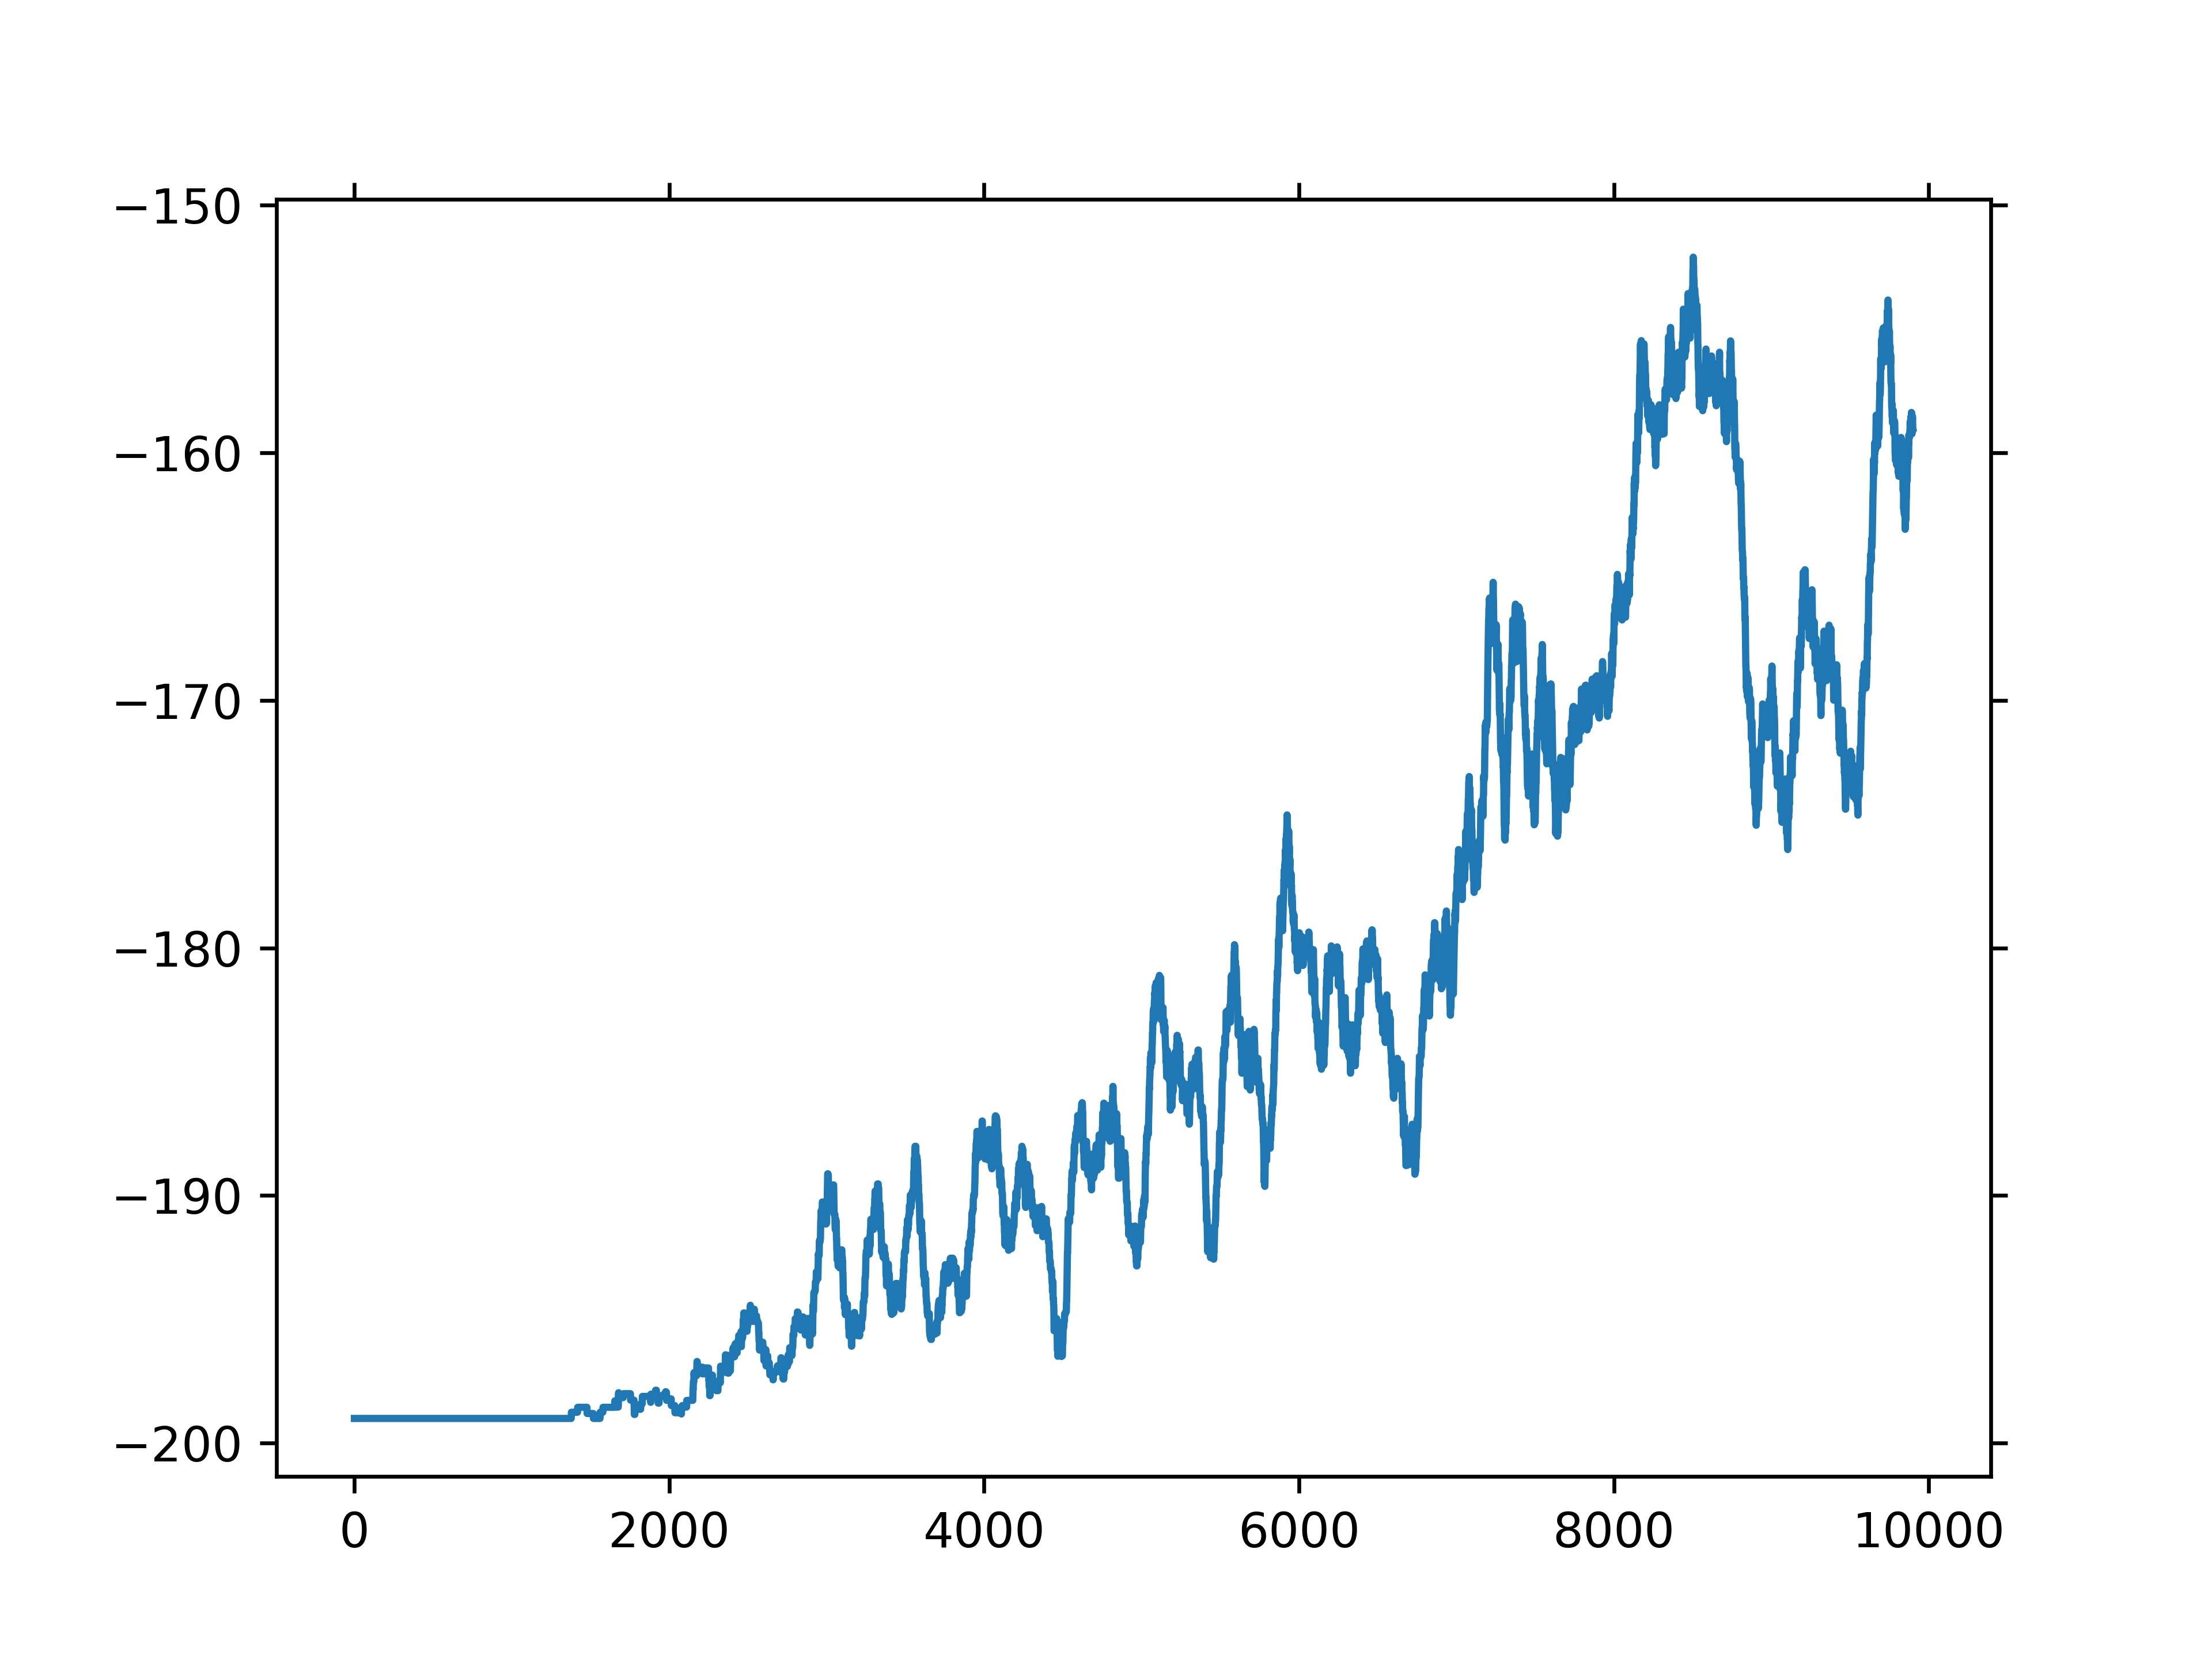
\includegraphics[width=0.7\linewidth]{T1.jpg}
        \caption{Tabular Sarsa(0) with $\epsilon=0.08$ and $\eta_{\,lr}=0.18$, i.e. it explores with $\epsilon$ probability and exploits with $1 - \epsilon$. In this case to discretize the state space we divide the entire range of positions and velocities into 50 uniform partitions. We return a \textbf{one-hot encoding} of the enabled partition index in the \mintinline[bgcolor=violet,
            frame=lines,
            framesep=2mm]{python}{get_table_features()} function.}
    \end{figure}%
    \textbf{Observations: } The idea of discretization in Tabular Sarsa(0) is pretty naive. Dividing the state space into non-intersecting blocks doesn't carry a lot of information. It takes around $\mathbf{164s}$ to converge and we receive a mean test reward of $\mathbf{-141.22}$ over 100 episodes. We also found this strategy to be very sensitive to the hyper-parameters $\epsilon$ and $\eta_{\,lr}$.
    
    \clearpage
    \section{\texttt{Task 2: Sarsa with Linear Function Approximation}}
    
    \begin{figure}[htbp!]
        \centering
        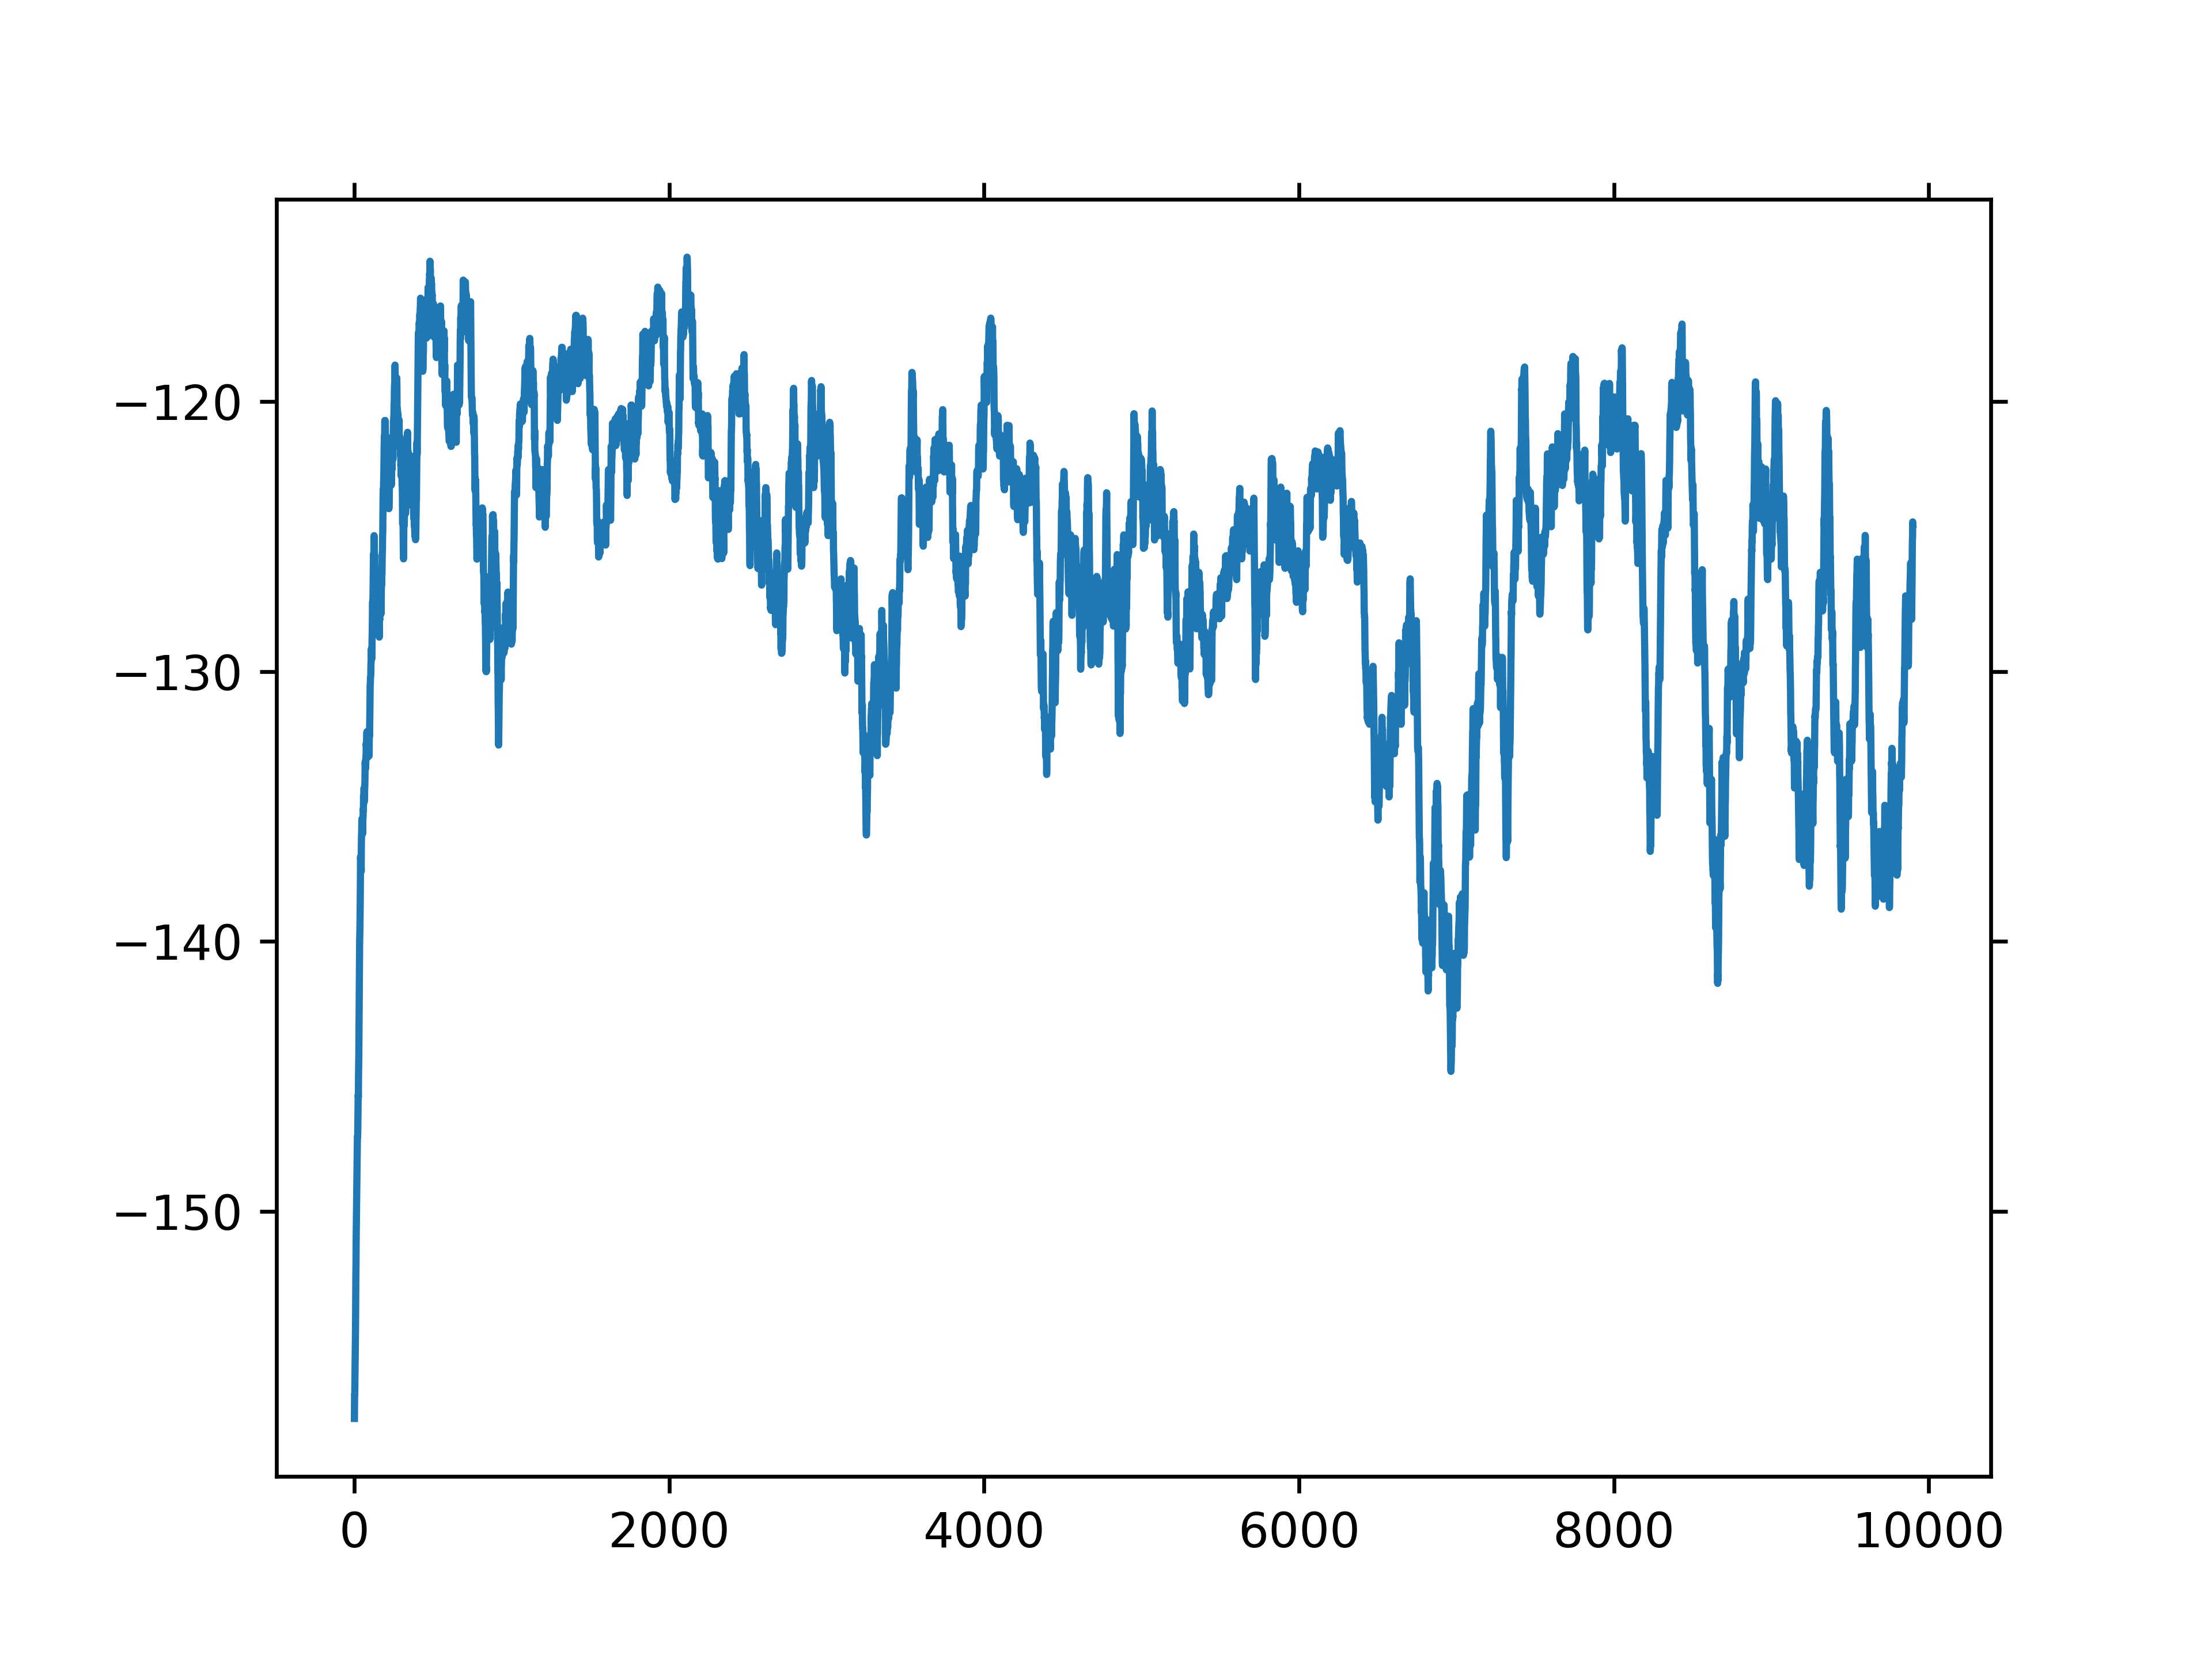
\includegraphics[width=0.7\linewidth]{T2.jpg}
        \caption{
            Sarsa(0) linear function approximation with RBF kernel. $\epsilon=0.05$ and $\eta_{\,lr}=0.18$. In this case we discretize the space with the same idea as before, i.e. 20 uniform partitions of the entire range of position and velocity. In this case instead of returning a one-hot encoding of the enabled partition index, we apply an $\mathbf{RBF}$ kernel on it. It is intuitive to provide some importance to the neighbouring $\mathbf{(x,v)}$ blocks (since we may want to assume, there won't be any drastic changes if the position or velocity of the car is changed slightly!). This sort of gives us a smoothened version of the one-hot encoding, which we return from the \mintinline[bgcolor=violet,frame=lines, framesep=2mm]{python}{get_better_features()} function.}
    \end{figure}%
    Say from a one-hot encoding like this:
    \begin{equation*}
        \begin{bmatrix}
            0 & 0 & 0 \\
            0 & 0 & 1 \\
            0 & 0 & 0
        \end{bmatrix}
        \longrightarrow
        \begin{bmatrix}
            0 & 0 & 0 & 0 & 0 & 1 & 0 & 0 & 0
        \end{bmatrix}
    \end{equation*}

    To this:
    \begin{equation*}
        \begin{bmatrix}
            0.08 & 0.37 & 0.61 \\
            0.14 & 0.61 & 1    \\
            0.08 & 0.37 & 0.61
        \end{bmatrix}
        \longrightarrow
        \begin{bmatrix}
            0.08 & 0.37 & 0.61 & 0.14 & 0.61 & 1 & 0.08 & 0.37 & 0.61
        \end{bmatrix}
    \end{equation*}
    
        
    \textbf{Observations: } This idea generalises very well for this problem setting! Our idea that there won't be any drastic changes if the position or velocity of the car is changed slightly, fits well in this setting. Upon careful vectorization of the RBF kernel operation, we observe faster convergence (particularly because of faster termination of the episodic task) than Tabular Sarsa(0) at $\mathbf{141s}$ with a mean test reward of $\mathbf{-104.03}$ over 100 episodes. If we take a look at the graph, its easy to observe that even below $\mathbf{1000}$ training iterations this method achieves much better results than Tabular Sarsa(0) at 10000 iterations.
    
    
\end{document}









